\documentclass[10pt,a4paper]{report}
\usepackage[utf8]{inputenc}
\usepackage{amsmath}
\usepackage{amsfonts}
\usepackage{amssymb}
\usepackage{cite}
\usepackage{url}
\usepackage{graphicx}

\newcommand{\bfx}{\mathbf{x}}

\begin{document}
\author{Marco De Mattia}
\title{Linearized Track Fitting}
\maketitle

\abstract

We present a method to perform a fast estimate of track parameters. We discuss the effect of a realistic detector considering the phase 2 tracker of the CMS experiment and we show how to correct for them. We conclude that a single linear approximation can be utilized over the full barrel region of the CMS tracker improving significantly over previous attempts that relied on segmenting the tracker in thousands of independent regions.

\section{Introduction}

The task of fitting tracks from a multitude of hits in the CMS silicon tracker is achieved offline by the CMS tracking software. The software uses a Kalman Filter approach to refine the information from hits in successive layers. Even in the offline environment, where time is in principle not a constraint, it is not feasible to explore all possible hit combinations. Seeds are instead built using layers that give 3D information (pixels, or double sided strip layers) to guide the search for hits in a narrower window. Even with this approach it is not feasible to perform track fitting within the 12.5 $\mu$s latency that will be available in the L1 trigger of CMS for the HL-LHC. New solutions must be found to reduce combinatorics and speed up the track fitting. One possible approach is to utilize associative memories (AM) to quickly group together subsets of the hits in roads that are potentially consistent with tracks. The coarsness of this step leads to multiple fake roads and an additional step is needed to refine the information, remove fakes, and estimate track parameters.

In this document we explore a method of fitting tracks out of a set of hits that is simple enough to be fast and implementable in FPGAs. This approach is based on a linear approximation of the dependence of the track parameters on the hit coordinates. The linear approximation will be acceptable only in a limited region of the phase space, i.e. an expansion of the function around a specific point. This method was utilized in the SVT at CDF and a review can be found in~\cite{SVTReview} and~\cite{SVTReviewFermilab}.

Other methods for track fitting at L1 trigger are being explored for CMS, such as Hough Transform and Retina Fit. They are not described in this document.

\section{Linear Approximation}

Each candidate track is represented as a list of $n$ hit coordinates, and can be thought of as a point $\mathbf{x}$ within a set $\mathcal{C} \subset R^n$. This subset is limited by the physical boundaries on the hit coordinates. Of all the points in $\mathcal{C}$ only a subset $\mathcal{T} \subset \mathcal{C}$ can be reasonably consistent with tracks coordinates. The concrete subset $\mathcal{T}$ is defined by specific criteria, such as a $\chi^2$ cut. Track finding is the process of deciding whether a set of coordinates corresponds to a track in $\mathcal{T}$.

Each track is fully defined by a set of $m < n$ parameters $\mathbf{p}$ (e.g. $p_T$, $\phi$, $\eta$, $d_0$, $z_0$). In the case of perfect detector resolution, the hit coordinates are uniquely determined by the parameters $\mathbf{p}$, and the set $\mathcal{T}$ reduces to an $m$-dimensional surface contained in $\mathcal{C}$, described by $n$ parametric equations,
\begin{equation}
\mathbf{x} = \mathbf{x}(p_1, \dots, p_m)\, .
\label{eq:x(p)}
\end{equation}
By eliminating the parameters equation~\ref{eq:x(p)} can be rewritten as $n - m$ constraint equations,
\begin{equation}
f_i(\mathbf{x}) = 0;\ i = 1, \dots, n-m\, .
\label{eq:constraints}
\end{equation}
A set of coordinates $\mathbf{x}$ corresponds to a track in $\mathcal{T}$ if and only if it satisfies the constraints equations.

In the case of finite detector resolution each hit coordinate has an associated uncertainty. The constraint functions ${f_i}$ then become random variables that take values slightly different from zero. Geometrically, the surface $\mathcal{T}$ acquires some thickness. In this case, there is no general exact solution to the constraint equations.

\subsection{Linearized Constraints}

The starting system of equations is generally not diagonal. However, given that the ${f_i}$ are random variables we can write their covariance matrix
\begin{equation}
F_{ij} = E[\ (f_i(\bfx) - E[f_i(\bfx)])(f_j(\bfx) - E[f_j(\bfx)]\ ]\, ,
\end{equation}
where $E[\ ]$ denotes the expected value. By expanding the constraint functions to first order around a point $\mathbf{x_0}$, and defining $\Delta x_r = x_r - x_{r0}$,
\begin{equation}
f_i(\bfx) \simeq \frac{\partial f_i}{\partial \bfx}(\bfx_0)\cdot (\bfx - \bfx_0) = \sum\limits_{r=1}^n \frac{\partial f_i}{\partial x_r}(\bfx_0)\Delta x_r\, ,
\end{equation}
we can express, to first order, the covariance matrix of the constraint functions {$f$} as a function of the covariance matrix of the deltas of the coordinates:
\begin{equation}
\begin{aligned}
F_{ij} &= E\left[\frac{\partial f_i}{\partial \bfx}(\bfx_0)\cdot (\bfx - \bfx_0) - E\left[\frac{\partial f_j}{\partial \bfx}(\bfx_0)\cdot (\bfx - \bfx_0) \right] \right] = \\
       &= \sum\limits_{rs}\frac{\partial f_i}{\partial x_r}\frac{\partial f_j}{\partial x_s} \ E\left[(\Delta x_r - E[\Delta x_r])(\Delta x_s - E[\Delta x_s])\right] = \\
       &= \sum\limits_{rs}\frac{\partial f_i}{\partial x_r}\frac{\partial f_j}{\partial x_s} \mbox{Cov}(\Delta x_r, \Delta x_s)
\end{aligned}
\end{equation}
The matrix $F_{ij}$ is a covariance matrix, therefore it is symmetric and it can be diagonalized through a rotation in the space of the $f_i$s. The new coordinates $\tilde{f}_i$ can be scaled to unit variance so that the sum $\sum_i \tilde{f}^2_i$, with $\langle\tilde{f}^2_i\rangle = 1$, follows a $\chi^2$ distribution as long as the PDFs of the $\tilde{f}_i$s are gaussian. The linear expansion of the diagonalized base of $\tilde{f}_i$s can be written as
\begin{equation}
\tilde{f}_i \simeq \frac{\partial \tilde{f}_i}{\partial \bfx}\cdot(\bfx - \bfx_0) = \mathbf{v_i} \cdot \bfx + c_i \, .
\label{eq:vis}
\end{equation}
Geometrically, this corresponds to approximating $\mathcal{T}$ with its tangent hyperplane in $\bfx_0$. The approximation will only work in a small region around $\bfx_0$, therefore, to apply this method over a large region and retain good accuracy the region must be split in smaller parts where the linearization is performed.

In principle, one can derive the constraint functions analytically given the detector geometry, magnetic field, and material. In practice, however, these functions can be arbitrarily complicated and determining their derivatives from first principles might not be practical. A numerical method can be used to estimate the linearized constraints via the empirical covariance matrix. If we sample directly the phase space of $\mathcal{T}$ we can build this covariance matrix and study its principal components, some of which are the $\mathbf{v_i}$s of equation~\ref{eq:vis}. We can do this by taking a sample of tracks (either from MC or from data), which by construction are sets of hits that belong to $\mathcal{T}$, and by computing the covariance matrix of their hit coordinates
\begin{equation}
\mbox{M}_{ij} \simeq E[ (\Delta x_i - E[\Delta x_i])(\Delta x_j - E[\Delta x_j])]\, .
\end{equation}
Diagonalizing this matrix, i.e. finding the principal components, will allow to estimate the $\mathbf{v_i}$s. Note that the full correlation matrix of the coordinates contains more information than the constraints, since it has a higher dimensionality ($n$) than the constraints covariance matrix ($n - m$). In general, what one obtains are $n$ eigenvectors and $n$ corresponding eigenvalues. Of these eigenvalues $m$ will be bigger than the others as their associated variances correspond to the dependence of the track parameters on the hit coordinates. Geometrically, their associated eigenvectors form a base on the hyperplane tangent to the surface $\mathcal{T}$ in $\bfx_0$. The remaining $n - m$ eigenvalues are smaller and correspond to the linearized constraints. Geometrically, their associated eigenvectors correspond to the coordinates perpendicular to the tangent hyperplane associated to the thickness of the surface $\mathcal{T}$ due to the finite detector resolution (uncertainties on the hit coordinates). We can take the $n - m$ eigenvectors with smaller eigenvalues, scale them to unit variance, and identify them with the $\tilde{f}_i$s. The advantages of this procedure are in its simplicity and in the possibility to perform it directly on data samples, thereby automatically accounting for possible detector misalignements and avoiding uncertainties that might affect the simulation.

With this method we can derive the coefficients $\mathbf{v_i}$ of the linearized constraints through which we can evaluate a $\chi^2$ for each set of hits.

\subsection{Linearized Track Parameters}

The method described in the previous subsection naturally yields a subset of $m$ eigenvectors that are associated to bigger eigenvalues and that can be related to the track parameters. However, these track parameters are not in a readily usable form (e.g. $p_T$, $\eta$, $\phi$, $d_0$ and $z_0$). We want to find the transformation from the principal components of the hit coordinates to the track parameters in a usable form. We can invert, at least locally, equation~\ref{eq:x(p)} to express the  parameters as a function of the hit coordinates
\begin{equation}
p_i = p_i(\bfx) \, .
\end{equation}
We consider a linear approximation of this equation in the form
\begin{equation}
p_i \simeq \mathbf{w_i}\cdot(\bfx - \bfx_0) + p_i(\bfx_0)
\end{equation}
or
\begin{equation}
\Delta p_i \simeq \mathbf{w_i} \cdot \mathbf{\Delta} \bfx = \sum\limits_{j=1}^n D_{ij} \Delta x_j
\end{equation}
where we defined $\Delta p_i = p_i - p_i(\bfx_0)$ and where $D_{ij}$ for $j\in [1,n]$ are the components of $\mathbf{w_i}$.
The best coefficients $D_{ij}$ are those that minimize the variance. We can estimate them on a sample of tracks using the least squares method and minimizing the sum of the squares of the deviations
\begin{equation}
\chi^2 = \sum\limits_{ik}\left(\sum\limits_j D_{ij} \Delta x_j^{(k)} - \Delta p_i^{(k)} \right)^2 \, ,
\label{eq:chi2}
\end{equation}
where the index $(k)$ denotes iteration on the tracks. Note that, unlike for the linearized constraints coefficients that could be derived also on data, this method can only be applied on MC because we need to know the true values of $\Delta p_i^{(k)}$

Equation~\ref{eq:chi2} presents a global $\chi^2 = \sum_i \chi^2_i$ computed using the deviations for all track parameters. Each parameter is estimated through a separate linear equation and these equations are independent. Therefore, minimizing the $\chi^2$ in equation~\ref{eq:chi2} is equivalent to minimizing the $\chi^2_i$ independently for each track parameter, and we only write it as a single value for convenience. This is important because the uncertainties between different tracks ($k$) can be assumed to be the same ($\sigma_{(k)} = \sigma$ for all $k$) and in this case the least squares expression above is equivalent to a $\chi^2$ (if the errors are also gaussian) apart from a multiplicative factor $1/\sigma^2$ which does not affect the result of the minimization. Furthermore, the errors have expectation zero, are uncorrelated and have equal variances as they all have the same $\sigma$, therefore from the Gauss-Markov theorem~\cite{GaussMarkov}, we know that the ordinary least squares estimator is the best linear unbiased estimator of the coefficients. In this case best means giving the lowest variance of the estimate.

To find the coefficients that minimize the $\chi^2$ let us consider the derivative
% \begin{equation}
% \begin{aligned}
% \frac12\frac{\partial \chi^2}{\partial D_{rs}} &= \sum\limits_{ik}\left(\sum\limits_j D_{ij} \Delta x_j^{(k)} - \Delta p_i^{(k)}\right) \sum\limits_q\delta_{ir}\delta_{qs}\Delta x_q^{(k)} = \\
% &= \sum\limits_{ik}\left(\sum\limits_j D_{ij} \Delta x_j^{(k)} - \Delta p_i^{(k)}\right) \delta_{ir}\Delta x_s^{(k)} = \\
% &= \sum\limits_k\left(\sum\limits_j D_{rj} \Delta x_j^{(k)} - \Delta p_r^{(k)}\right) \Delta x_s^{(k)} \, .
% \end{aligned}
% \end{equation}
\begin{equation}
\begin{aligned}
\frac12\frac{\partial \chi^2}{\partial D_{rs}} &= \sum\limits_{ik}\left(\sum\limits_j D_{ij} \Delta x_j^{(k)} - \Delta p_i^{(k)}\right) \sum\limits_q\delta_{ir}\delta_{qs}\Delta x_q^{(k)} = \\
&= \sum\limits_k\left(\sum\limits_j D_{rj} \Delta x_j^{(k)} - \Delta p_r^{(k)}\right) \Delta x_s^{(k)} \, .
\end{aligned}
\end{equation}
By solving the equation obtained by setting the derivative equal to zero we can find the best coefficients. We have
\begin{equation}
\sum\limits_j D_{rj} \sum\limits_k \Delta x_j^{(k)} \Delta x_s^{(k)} = \sum\limits_k \Delta p_r^{(k)} \Delta x_s^{(k)} \, .
\label{eq:D}
\end{equation}
Given $N$ tracks, the second half of equation~\ref{eq:D} is $N-1$-times the element $C^{(p)}_{rs}$ in the empirical correlation matrix between track parameters and hit coordinates (where $x_0$ and $p_0$ are taken as the expected values, or the means) since
\begin{equation}
C^{(p)}_{rs} = \sum\limits_{k=1}^N \frac{\Delta p_r^{(k)} \Delta x_s^{(k)}}{N-1} \, ,
\end{equation}
and part of the left term is $N-1$-times the empirical covariance matrix of the hit coordinates $C^{(v)}_{js}$ since
\begin{equation}
C^{(v)}_{js} = \sum\limits_{k=1}^N \frac{\Delta x_j^{(k)} \Delta x_s^{(k)}}{N-1} \, .
\end{equation}
We can finally write
\begin{equation}
\sum\limits_j D_{rj} C^{(v)}_{js} = C^{(p)}_{rs} \, ,
\end{equation}
or in matrix form
\begin{equation}
D\cdot C^{(v)} = C^{(p)}
\end{equation}

We conclude that the matrix $D$ that performs the linear transformation from the hit coordinates to the track parameters and with coefficients that minimize the variances can be obtained from the covariance matrix of the hit coordinates and from the correlation matrix between track parameters and hit coordinates as
\begin{equation}
D = C^{(p)} \cdot C^{(v)-1} \, .
\label{eg:Dfinal}
\end{equation}
This result is valid independently of the form of the correlation matrix $C^{(v)}$. However, if it is diagonal, i.e. if we are in the base of the principal components, then the inverse matrix $C^{(v)-1}$ is still diagonal with elements $1/\lambda_{ii}$ on the main diagonal, where $\lambda_{ii}$ are the eigenvalues of $C^{(v)}$. In this case equation~\ref{eg:Dfinal} simplifies to
\begin{equation}
D_{ij} = \sum\limits_r C^{(p)}_{ij}/\lambda_{jj}\, , \, \, \mbox{for } i,j \in [1,n] \, .
\end{equation}


\section{Application to the CMS Detector}

We apply the method described in the previous section to the silicon strip tracker for the phase 2 upgrade of the CMS detector. In this application we will focus on the barrel region which consists of six layers. For a 3D fit we have three coordinates per layer and with six layers we have a total of 18 coordinates. The barrel region has a cylindrical symmetry, we therefore utilize the cylindrical coordinates ($\phi, R, z$) to describe the positions of the hits. The trajectory of a charged particle in a uniform magnetic field can be described by a helix (neglecting energy loss effects) and requires 5 parameters. We take these parameters to be
\begin{itemize}
\item $c/p_T$: the charge over the transverse momentum of the particle.
\item $phi_0$: the $phi$ angle of the momentum vector at the point of closest approach to the origin.
\item $d_0$: the transverse impact parameter, defined as the minimum distance between the trajectory and the origin in the transverse plane.
\item $cot(\theta)$: the cotangent of the angle between the momentum vector and the z axis (along which the magnetic field is directed) at the point where $d_0$ is evaluated.
\item $z_0$: the z coordinate of the trajectory at the point where $d_0$ is evaluated.
\end{itemize}
For a trajectory passing through the origin in the transverse plane ($d_0 = 0$) we can write the coordinate $\phi$ of a point on the trajectory as a function of its radius $R$ and of the track parameters $c/p_T$ and $\phi_0$ as:
\begin{equation}
\phi = \phi_0 - \mbox{arcsin}\left(\frac{R}{2\rho}\right)\, ,
\label{eq:trajectoryPhi}
\end{equation}
where
\begin{equation}
\rho = \frac{p_T}{0.003\cdot B\cdot c}
\end{equation}
is the curvature radius of the trajectory (radius of the circle deriving from the projection of the trajectory in the transverse plane) and is expressed in cm.

For a perfectly cylindrical detector the radial coordinates do not provide information useful for a principal component analysis of the hit correlations since it is a fixed value for each layer. It is sufficient to consider hits from different layers as separate inputs. In a real detector, however, the hit coordinates for a given layer will not be at the same radius because of two effects: the modules are flat, and they are staggered to allow for overlaps and detector hermeticity. In the following we will show that these effects are not negligible in the upgraded CMS tracker and we will provide a solution that allows to reduce the realistic detector to the ideal case of a perfect cylinder to a very good approximation.

\subsection{Effect of the Variation of the Module Radius Within a Layer}

Let us consider the first order expansion of equation~\ref{eq:trajectoryPhi}\footnote{This approximation is valid for small values of the $R/(2\rho)$. For a 2 GeV/c track $\rho \simeq 175$ cm and for the outermost layer the biggest radius is $\simeq 110$ cm. Therefore, $R/(2\rho) \simeq 0.31$. The second order term in the taylor expansion is $(R/(2\rho))^3/6 \simeq 0.005$ which is about 1.6\% of the first order term and should be corrected for low $p_T$ tracks. For a 3 GeV/c track the effect is about 0.15\%.}
\begin{equation}
\phi \simeq \phi_0 - \frac{R}{2\rho} \, .
\label{eq:trajectoryPhiLinearized}
\end{equation}
If we want to estimate the track parameters $\phi_0$ and $c/p_T$ with a linear combination of the $\phi$ coordinates of the hits in the detector layers we can write
\begin{align}
\phi_0 = \sum_i A_i \phi_i \, , \\
\frac{c}{p_T} = \sum_i B_i \phi_i \, ,
\label{eq:linearCombination}
\end{align}
and we know that the principal component analysis (PCA) can be used to derive optimal coefficients for these expressions (in the sense that they minimize the $\chi^2$). Substituting equation~\ref{eq:trajectoryPhiLinearized} we obtain
\begin{align}
\phi_0 \simeq \phi_0\sum_i A_i + \frac{1}{2\rho}\sum_i A_i R_i\, , \\
\frac{c}{p_T} \simeq \phi_0\sum_i B_i + \frac{1}{2\rho}\sum_i B_i R_i \, ,
\end{align}
which yield the following constraints on the coefficients
\begin{align}
\sum_i A_i &= 1\, , \, \sum_i A_i R_i = 0\, , \\
\sum_i B_i &= 0\, , \, \sum_i B_i R_i = -\frac{2}{0.003\cdot B}\, .
\end{align}
In a perfectly cylindrical detector the $R_i$ are constant for each layer and it is possible to perfectly satisfy the constraints. In this case the PCA would provide the exact values of the coefficients that minimize the $\chi^2$. In a real detector, however, there are two effects that make it not possible to perfectly satisfy the constraints. The first effect is due to the modules being staggered to provide hermeticity to the detector. In the barrel the staggering is both along $\phi$ and along $z$ and it causes the radius of the hits to change when moving between adjacent modules. The second effect is due to the flatness of the modules which causes the distance from the hits to the origin to change along the surface of the module. These two effects are not negligible in the planned CMS tracker for the phase 2 upgrade and must be accounted for to achieve the best possible resolution. In the following we will focus our discussion on the $p_T$ resolution. Similar considerations apply to the $\phi_0$ and $d_0$ resolutions.

Figure~\ref{fig:quarterTransverseView} shows the structure of the transverse projection of a quarter of the barrel of the silicon strip tracker for the phase 2 upgrade of the CMS detector as simulated in the CMS software version CMSSW\_6\_1\_0\_SLHC20\_patch1. For each of the six layers it is possible to see pairs of modules at the same angle $\phi = \mbox{arctan}(y/x)$ which correspond to different $z$ positions. It is immediately clear that there is a significant variation in radius among adjacent modules and, to first order, that there are four different sets of radii for each layer. Considering all layers there are $4^6$ unique combinations of radii for the full silicon strip tracker. If one were to neglect the variations along $z$ there would be $2^6$ combinations.
\begin{figure}
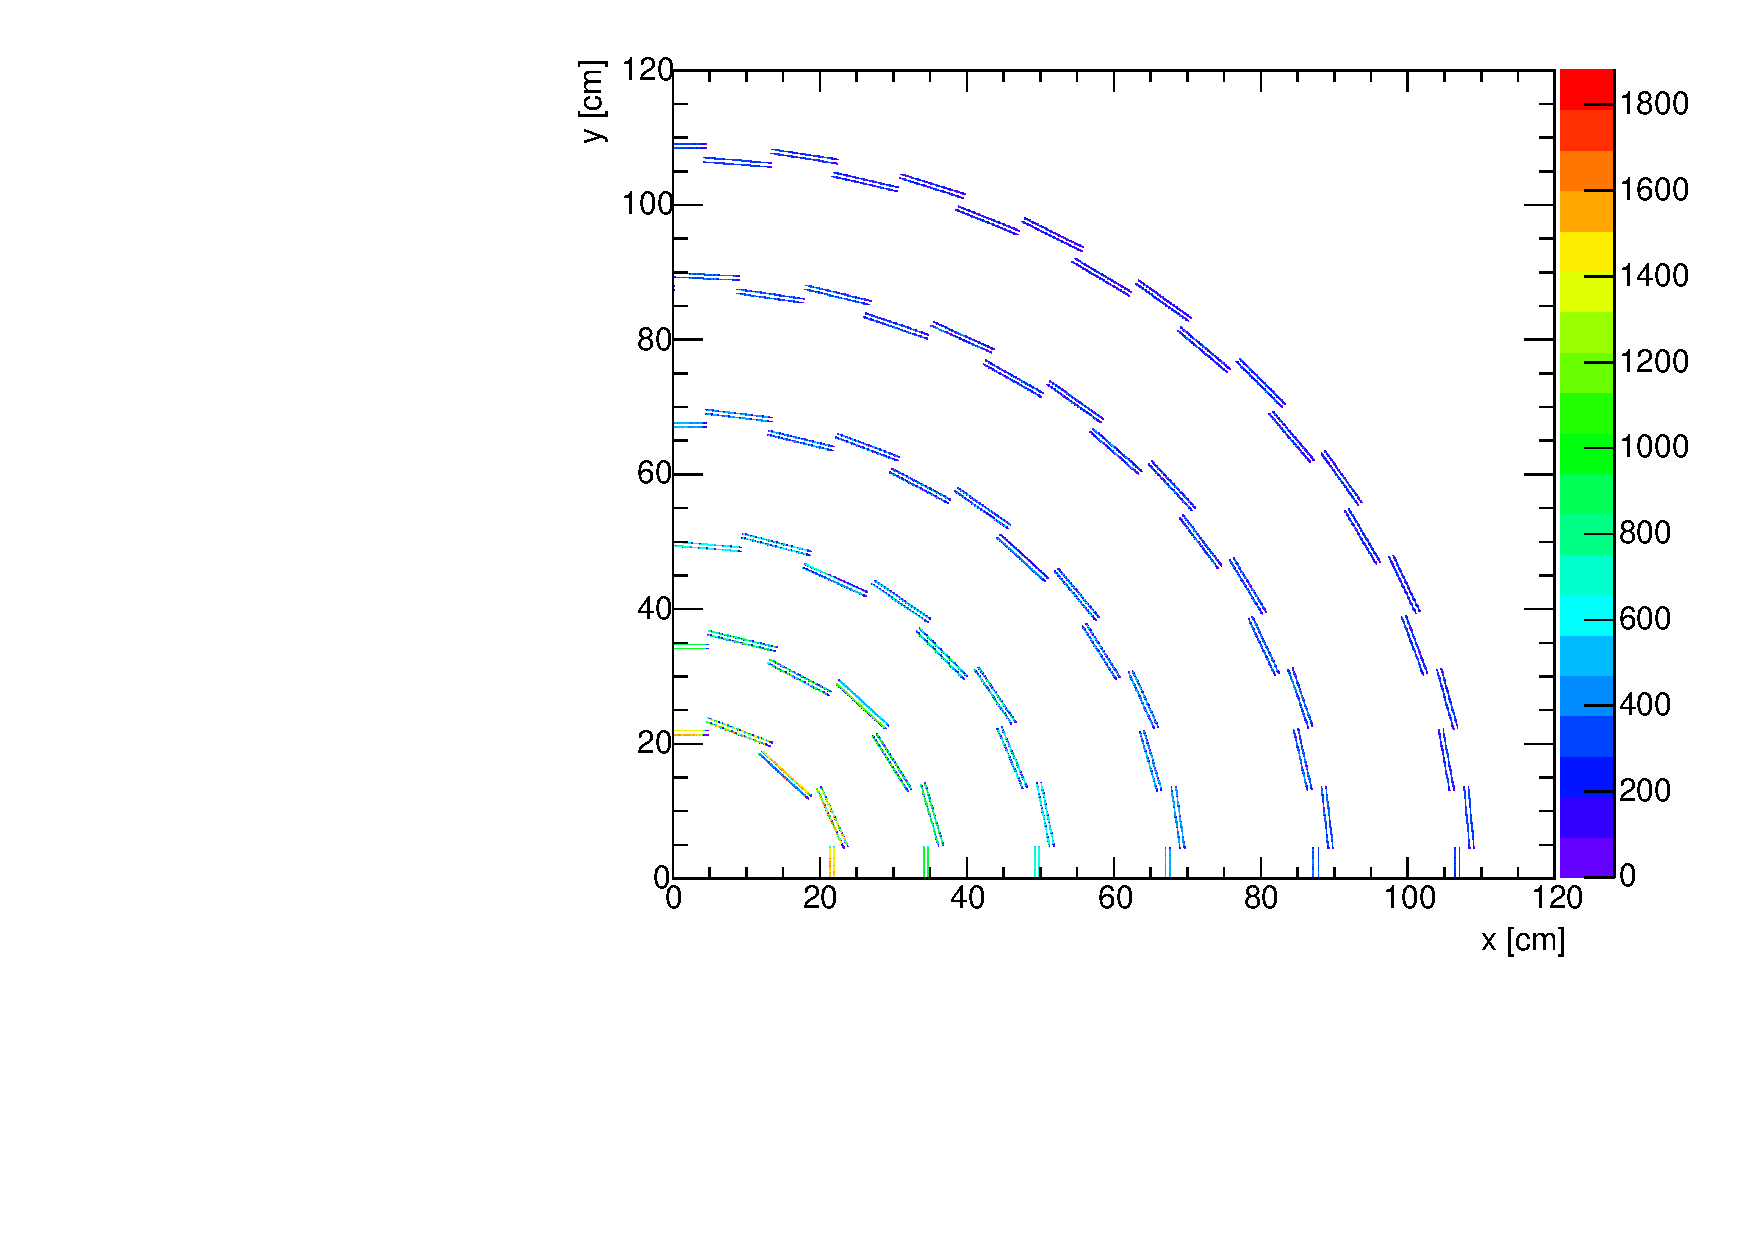
\includegraphics[width=\textwidth]{Figures/QuarterTransverseView.pdf}
\caption{A view of the modules in the transverse projection of a quarter of the barrel of the CMS silicon tracker for the phase 2 upgrade. The geometry utilized is the default in the CMS software version CMSSW\_6\_1\_0\_SLHC20\_patch1. The plot is obtained by generating single muons and showing the position of the stubs reconstructed by the emulation of the front-end electronic of the strip tracker. The color bar shows the number of entries.}
\label{fig:quarterTransverseView}
\end{figure}

Figure~\ref{fig:OutermostRadiusVariation} shows the variation in the $\phi$ coordinate of the hits  in the outermost layer produced by a 2 GeV/c track from the innermost to the outermost module in that layer. This variation is about 2.4\%. From equation~\ref{eq:trajectoryPhi} we can compute the $p_T$ of a track that would produce, on the outermost module, a hit with the same $\phi$ of the hit produced by the 2 GeV/c track in the innermost module. This relative variation in $p_T$ is approximately independent of $p_T$ and is approximately inversely proportional to the variation of the radius of the hit. The biggest variation is in the innermost layer where it can big as big as about 11\% while in the outermost layer it is the smallest and it is about 2.4\%.

An additional effect that causes biases and reduces the precision of the measured parameters is the module flatness, which causes a variation of the radius of the hit inside a single module. This effect is most important for the innermost layer, where 16 modules cover the full $\phi$ angle with each module covering approximately 0.4 radians. Assuming the center of the module to be its closest point to the origin and having a radius of approximately 23 cm, the radius at the edge is approximately 23.5 cm, a variation of about 2\%. For a 2 GeV/c track this translates in a similar effect on the $p_T$ of about 2\%. For the second innermost layer this effect is reduced to less than 1\% by the increase in the number of modules (24) and it is reduced further as the number of modules per layer increases.

The expected offline $p_T$ resolution in the upgraded tracker is about 0.5\% for a $p_T$ of 2 GeV/c and better than 2\% at high $p_T$ (around 100 GeV/c). It is clear that the effects discussed above would preclude the possibility of reaching this level of precision and they need to be corrected. Simulation studies show that the impact of the module flatness on the $p_T$ resolution is small. This can be understood from the fact that the effect is already smaller than 1\% in the second layer and decreases further in the outermost layers. Correcting for it can improve the $p_T$ resolution from 0.6\% to about 0.5\% (a 10-15\% relative increase). The effect of the module staggering, on the other hand, is as big as 11\% in the innermost layer and not smaller than 2\% in the outermost. Even assigning a bigger weight to the outermost layers the $p_T$ resolution would be limited to about 2\% at low $p_T$ (2 GeV/c) and it would be limited to about 3\% at high $p_T$ (100 GeV/c) (estimated as the sum in quadrature of the intrinsic resolution of the detector (about 2\%) and the effect of module staggering (about 2\%)). These numbers were verified with a full simulation of the upgraded CMS tracker using samples of single muons and anti-muons. In what follows we will describe a simple method to correct these effects that allows to achieve close to offline-like resolutions with a linearized fit.
\begin{figure}
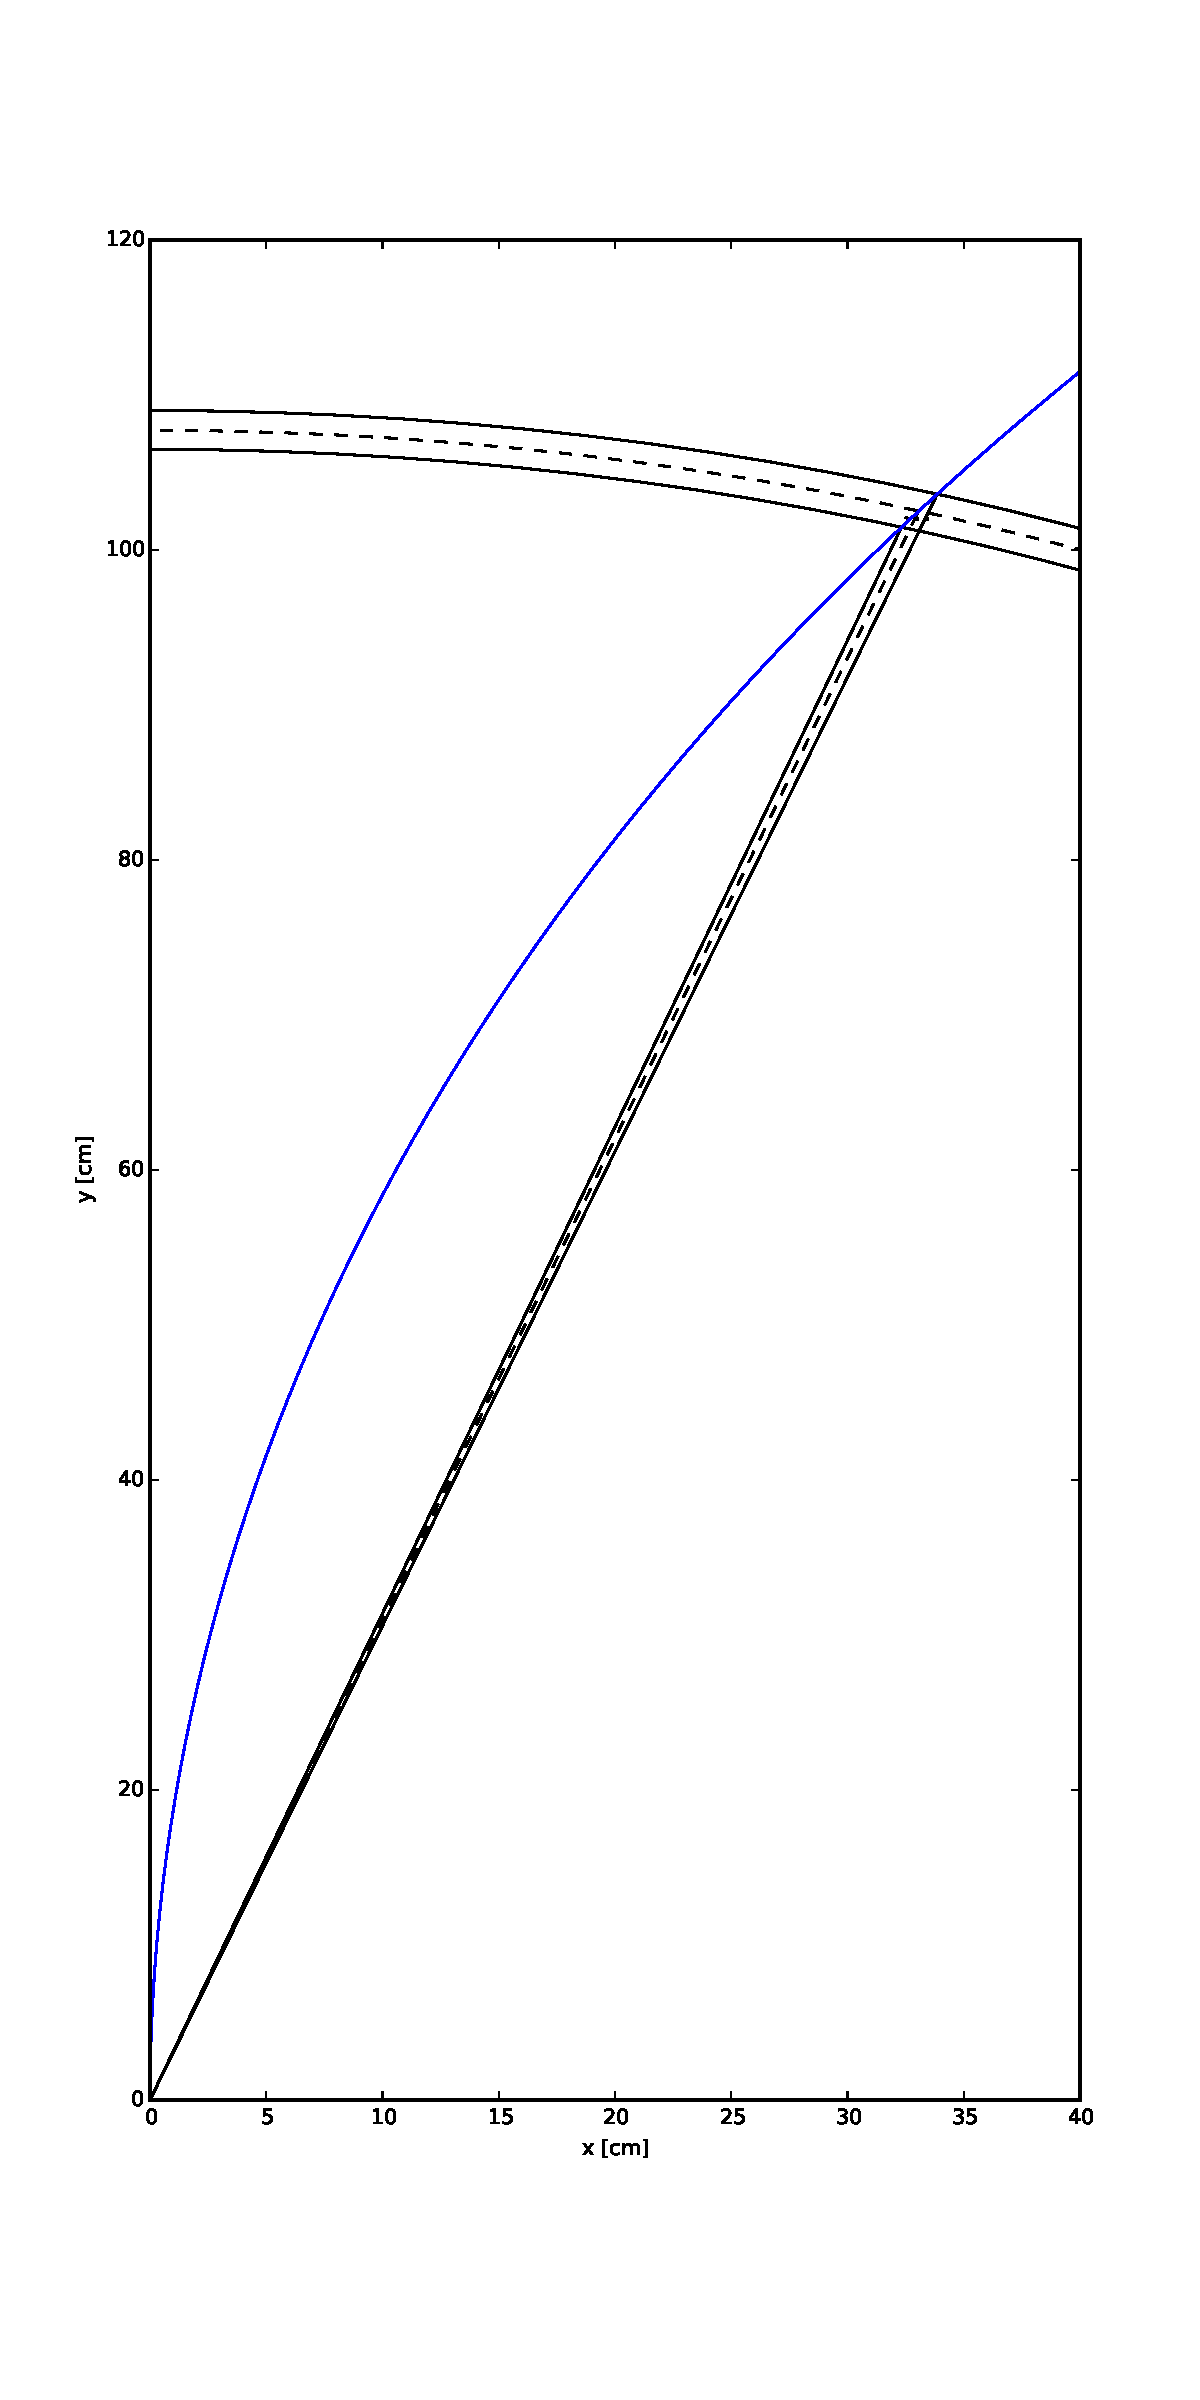
\includegraphics[width=0.45\textwidth]{Figures/OutermostRadiusVariation.pdf}
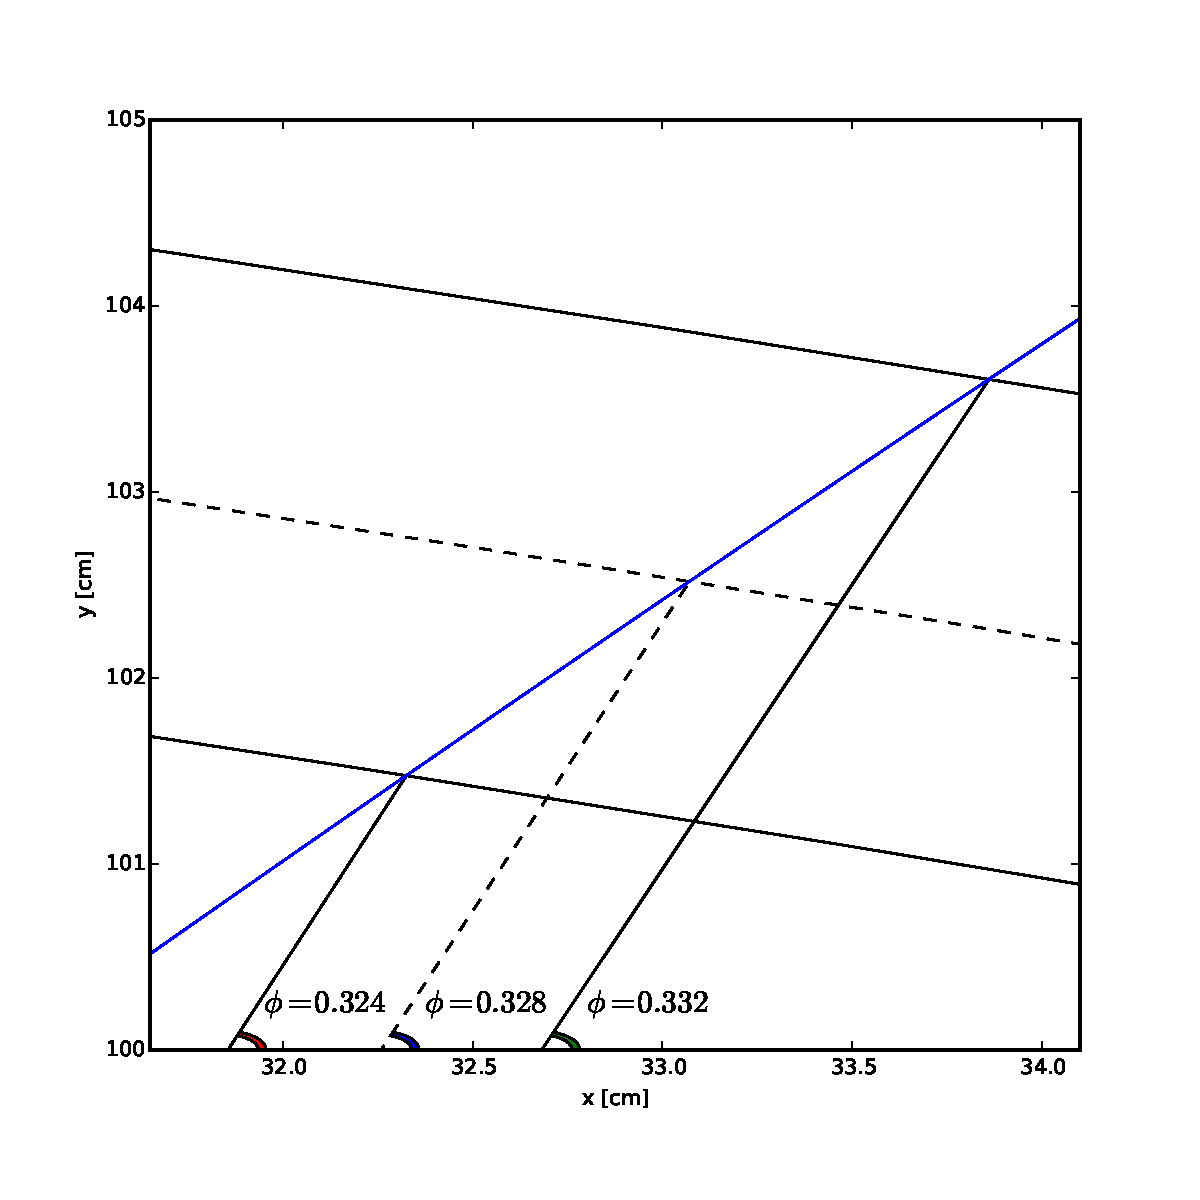
\includegraphics[width=0.45\textwidth]{Figures/OutermostRadiusVariationZoom.pdf}
\caption{(Left) Variation of the $\phi$ angle for the hits produced by a 2 GeV/c track crossing the outermost layer of the silicon strip tracker for the phase 2 upgrade of CMS. The internal and external curved lines show the average position of the innermost and outermost modules in the layer, while the dotted curved line shows the average position of all modules in the layer. (Right) Zoomed view of the left figure in the area of the hits. The $\phi$ angles show the $\phi$ coordinates of the hits that would be produced, from left to right, in the innermost module, a module in the average radius of all layer modules, and outermost module.}
\label{fig:OutermostRadiusVariation}
\end{figure}

\subsection{Correction of the $\phi$ Coordinates}

We describe a simple method to correct the $\phi$ coordinates for each layer for the variation of the radii. For each layer we take the average radius of all the modules as the radius of an ideal layer and we correct all the $\phi$ coordinates as if the hits were on this ideal layer. From equation~\ref{eq:trajectoryPhi} it is clear that the shift of the $\phi$ coordinate due to the change in radius is $p_T$-dependent. Therefore, we need to know the $p_T$ to be able to perform the correction. If the radius of the ideal layer is $R'$ we can write, to first order, the corrected $\phi'$ coordinate at the intersection of the track with this ideal layer as a function of the original $\phi$, $R$ and $\rho$ as
\begin{equation}
\phi' = \phi + \frac{R - R'}{2\rho}\, .
\end{equation}
The correction to the $\phi$ for the change in radius is generally of 1-2\%, as discussed in the previous section. Therefore, the value of the $c/p_T$ utilized for the correction can be obtained from a simpler, first order estimate and does not need to be extremely accurate, as will be explained below. To obtain this estimate we perform a first PCA analysis of the $\phi$ coordinates of the hits in a sample of tracks and derive a set of coefficients to estimate the $c/p_T$ from the $\phi$ of all the hits for a given track. From what we discussed in the previous section we know that the resolution of this preliminary estimate is about 2\% at low $p_T$ and order of 3\% at higher $p_T$ (around 100 GeV/c). This is enough as a pre-estimate because it allows to perform a correction on an approximately 2\% shift of the $\phi$ coordinates with a precision better than 3\%. We obtain a new set of corrected $\phi$ coordinates which we utilize for a second PCA analysis. The new set of coefficients allows for a much improved estimate of the track parameters. Full detector simulation studies show that it is possible to achieve close-to-offline levels of $p_T$ resolution (0.5\% at 2 GeV/c and better than 2\% at 100 GeV/c).

To perform the first estimate of the $c/p_T$ it is sufficient to store six coefficients as shown by equation~\ref{eq:linearCombination} and it would require six multiplications and five additions to compute. Applying the correction to each coordinate would require six more multiplications by the radii and the addition of the result to the $\phi$ coordinates. Furthermore, performing the correction restores cylindrical symmetry to the detector allowing to use a single set of PCA coefficients to estimate the $\chi^2$ and the final track parameters for the full $\phi$ and $\eta$ range in the barrel. This is a distinct advantage over other approaches that consider each possible combination of modules as a separate entity with a dedicated set of coefficients.

For low $p_T$ tracks a first order correction might not be enough since the non-linearity in the arcsin of equation~\ref{eq:trajectoryPhi} leads to a 1.6\% effect for a 2 GeV/c track (and a 0.15\% for a 3 GeV/c track). In this case there are two possible alternatives. The first one is to compute a dedicated set of constants for the 2-3 GeV/c $p_T$ range. The initial $c/p_T$ estimate allows to select the correct set of constants for this $p_T$ range and the limited range allows the PCA to optimize the corrections to compensate for the non-linearities. The second possibility is to correct the $\phi$ coordinates with the second order term in the taylor expansion of the arcsin, which would require a few additional operations per track.

\subsection{Correction of the $z$ Coordinates}

The same approach can be applied to the calculation of the $z_0$ and $\cot\theta$ parameters by considering the equation expressing the $z$ coordinate of the trajectory as a function of the track parameters and of the radius
\begin{equation}
z = z_0 + 2\rho\cdot\mbox{arcsin}\left(\frac{R}{2\rho}\right)\cot\theta\, ,
\end{equation}
and noting that its first order expansion of the arcsin around $R/(2\rho) \simeq 0$ is\footnote{The second order term is $\frac{1}{24}\frac{R^3}{\rho^2}\cot\theta$. The effect of this term is biggest for the lowest $p_T$ and for the larger radius. For a 2 GeV/c track the effect is 1.5\% at the outermost layer and 0.07\% at the innermost layer. For a 3 GeV/c track the effect is 0.6\% at the outermost layer and 0.03\% at the inmermost layer.}
\begin{equation}
z \simeq z_0 + R\cdot\cot\theta\, .
\end{equation}
The effect of the variation of the radii on the $\cot\theta$ is similar to the effect on $p_T$ in the case of the $\phi$ coordiantes. The effect is maximum in the outermost layer where it is about 11\% and minimum in the innermost layer where it is about 2.5\%. Again, this is a non-negligible effect and should be corrected to achieve a good performance with the linearized track fit. The same approach used for the $\phi$ coordinates can be applied to the $z$ coordinates by building a first order estimate of $\cot\theta$ utilizing only the $z$ coordinates and using it to compute corrected-$z$ coordinates referred to the ideal layers.

\section{The Disks}

The geometry of the CMS tracker is that of concentric cylindrical layers of modules in the so-called barrel and of modules arranged in disks in the so-called endcaps. So far we focused our discussion on the barrel component of the tracker. However, the algorithm described here can be applied with not change to a disk-based geometry, since it will perform an intermediate transformation that changes that geometry to a smooth barrel. The modules used in both barrel and endcaps have strip that are parallel to each other. In the endcaps the modules are arranged so that the strips roughly point back to the z axis. However, since they are parallel to each other, if one strip points to the z axis, all others will not. Since we do not have information on the position of the charge deposit along the strip, each stub on each strip in the disks is assigned the $R$ coordinate of the center of the strip. Figure~\ref{fig:NonRadialStrips} illustrates how the non-radial strips arrangement causes the correct $R$ of the stub to deviate from the assigned $R$ if the particle did not pass through the center of the strip. This deviation is roughly proportional to the distance from the center of the strip. As a consequence, the $\phi$ coordinate is also biased as shown in the figure.

\begin{figure}
\begin{center}
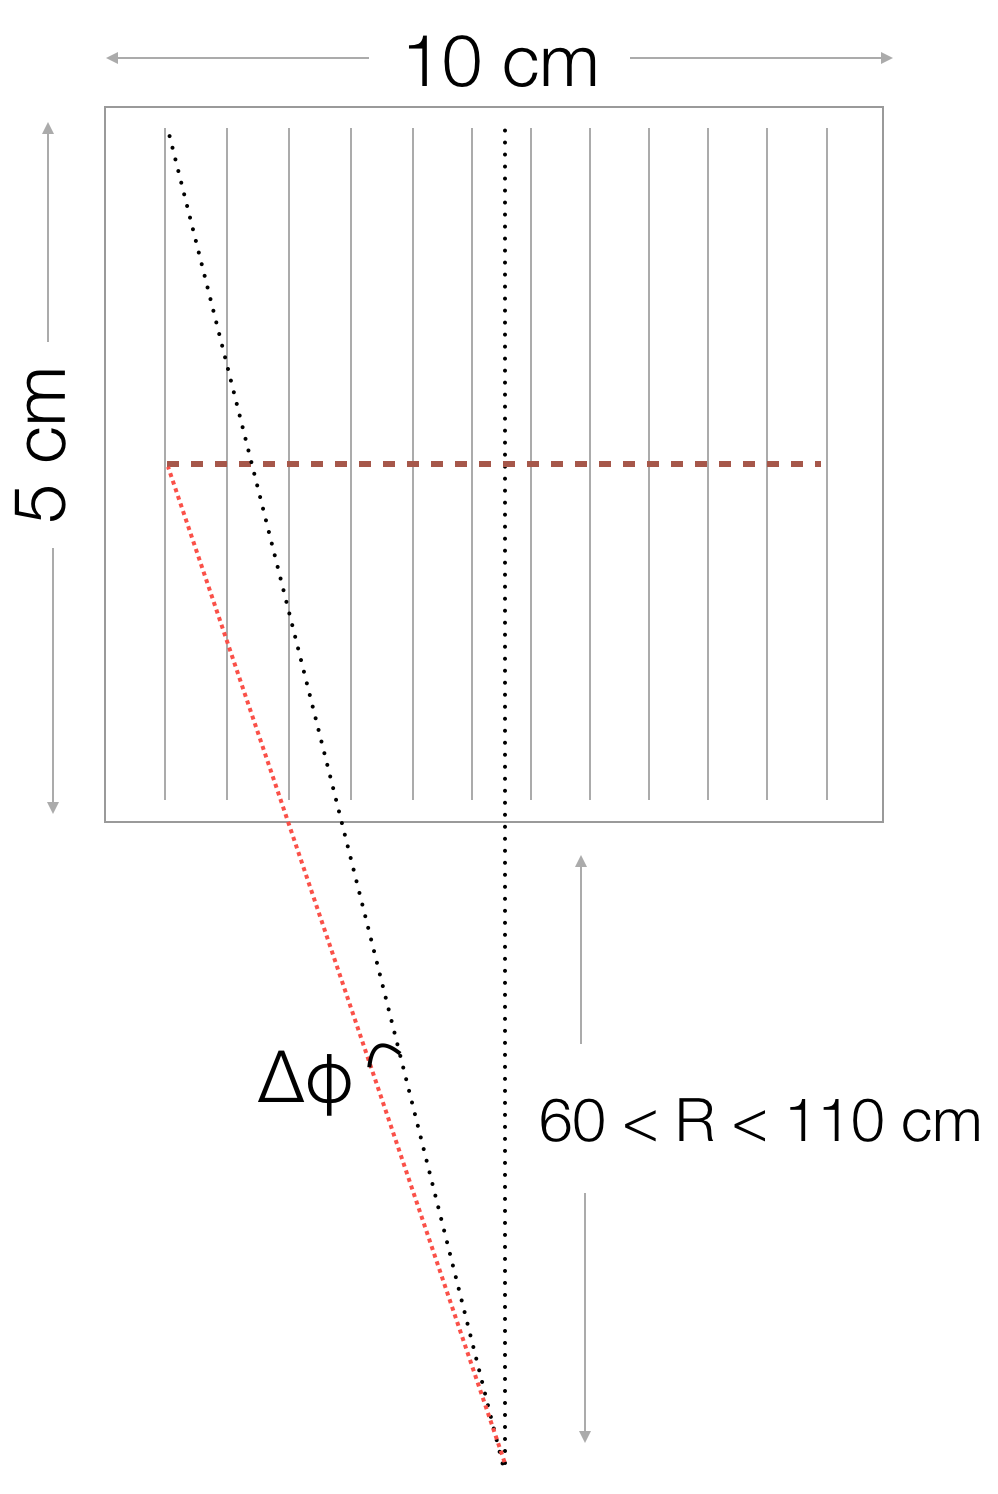
\includegraphics[width=0.45\textwidth]{Figures/NonRadialStrips.png}
\caption{Variation of the $\phi$ coordinate along the strip length due to the non-radial arrangement of the strips. This sizes shown are for strips in 2S modules.}
\label{fig:NonRadialStrips}
\end{center}
\end{figure}

While this effect is present for every strip in the disks that does not point back to the z axis, the effect is most important for 2S modules where the strips are 5 cm long. In the PS modules, the reduced strip length of 2.5 mm makes the effect negligible.

To correct for this effect we need to have a better estimate of the position of the stub along the strip. Since in the innermost modules are from PS modules that have a much better resolution along $R$ than the 2S modules, we extrapolate the trajectory linearly from the outermost PS module to the 2S modules in the disks. We then correct the $\phi$ coordinate with (to first order):
\begin{equation}
\Delta\phi \approx \mbox{pitch} \cdot (\mbox{strip\_index} - \mbox{central\_index}) \cdot \frac{R_{extrapolated} - R}{R^2} \, ,
\end{equation}
where
\begin{itemize}
\item pitch = 90 $\mu$m;
\item strip\_index is the index of the strip from 0 to 1015;
\item central\_index = 507.5. This is the index a strip would have if placed at the center of the module.
\end{itemize}
And the $R_{extrapolated}$ is computed to second order approximation as
\begin{equation}
R_{extrapolated} \approx R + \Delta z \tan\theta + \left(\frac{1}{2\rho}\right)^2 \cdot \left(-\frac12R^2 \cdot \Delta z \tan \theta - \frac12 R \cdot (\Delta z\tan \theta)^2 - \frac16 (\Delta z \tan \theta)^3\right) \, .
\end{equation}


\subsection{Conclusions}

A method to compute optimal coefficients for a linear estimate of the track parameters using a principal component analysis was presented. It was shown that the effect of the variation of the radii of modules in a layer of the CMS tracker for the phase 2 upgrade has a non-negligible impact on the accuracy of this linear estimate. A simple method to correct this effect in the barrel was also presented. Overall, a single set of PCA coefficients is enough to provide performance close to the offline reconstruction over the full barrel. Splitting the PCA coefficients in few $p_T$ regions can further improve the performance by reducing the effect of non-linearities at low $p_T$.

\newpage
\appendix
\section{One-Pass Evaluation of Mean and Covariance}

The mean of a random variable $x$ over a sample of size $N$ can be defined as
\begin{equation}
\bar{x}_N = \sum\limits_{i=1}^N\frac{x_i}{N}\, ,
\label{eq:mean}
\end{equation}
and the covariance for two random variables $x$ and $y$ can be estimated with the empirical covariance matrix in a sample of size $N$
\begin{equation}
\mbox{Cov}(x,y) = \sum\limits_{k=1}^N \frac{(x_i - \bar{x}_N)(y_i - \bar{y}_N)}{N-1}\, ,
\label{eq:covariance}
\end{equation}
where the $N-1$ at denominator makes the estimator unbiased given that we evaluate the mean from the same sample.

Evaluating the mean and covariance of a large sample using these formulas is not practical since one would need to know the total size of the sample for computing the mean and the mean itself for computing the covariance. This implies having to iterate over the sample more than once. Furthermore, the formula for the mean is not numerically stable, since the sum at numerator can be arbitrarily big. Iterative formulas for evaluating both mean and covariance will be derived in this section. For a reference to these, and more general formulas which allow to split the calculation in arbitrary number of parts and combine the results, useful for parallelizing the evaluation, see~\cite{IterativeMeanAndCovariance}.

First of all, let us derive an iterative formula for computing the mean in one pass. From equation~\ref{eq:mean} we can write
\begin{equation}
\bar{x}_N = \frac{N-1}{N}\sum\limits_{i=1}^{N-1}\frac{x_i}{N-1} + \frac{x_N}{N} = \frac{N-1}{N}\bar{x}_{N-1} + \frac{x_N}{N}\, ,
\label{eq:iterativeMean}
\end{equation}
or, in a format convenient for C++,
\begin{equation}
\bar{x}_{N-1} \mathrel{+}= \frac{x_N - \bar{x}_{N-1}}{N} \, .
\end{equation}

We can use the result of equation~\ref{eq:iterativeMean} for deriving the iterative formula for the empirical covariance matrix. It is more terse to derive a recursive formula for $\mathcal{M}(x,y)$ defined as
\begin{equation}
\mathcal{M}_N(x,y) = (N-1)\cdot\mbox{C}_N(x,y) = \sum\limits_{k=1}^N (x_i - \bar{x}_N)(y_i - \bar{y}_N)\, ,
\label{eq:coMoment}
\end{equation}
where $\mbox{C}_N$ denotes that the empirical covariance matrix is evaluated on a sample of size $N$. Utilizing equation~\ref{eq:iterativeMean} in equation~\ref{eq:coMoment} we have
\begin{equation}
\begin{aligned}
\mathcal{M}_N(x,y) =& \sum\limits_{i=1}^{N-1}(x_i - \bar{x}_N)(y_i - \bar{y}_N) + (x_N - \bar{x}_N)(y_i - \bar{y}_N) = \\
=& \sum\limits_{i=1}^{N-1}\left(x_i - \bar{x}_{N-1} - \frac{x_N - \bar{x}_{N-1}}{N}\right)\left(y_i - \bar{y}_{N-1} - \frac{y_N - \bar{y}_{N-1}}{N}\right) +\\
&+ \frac{N-1}{N}(x_N - \bar{x}_{N-1})(y_N - \bar{y}_N) = \\
=& \ \mathcal{M}_{N-1}(x,y) + \sum\limits_{i=1}^{N-1}(x_i-\bar{x}_{N-1})\left(\frac{\bar{y}_{N-1} - y_N}{N}\right) +\\
&+ \sum\limits_{i=1}^{N-1}(y_i-\bar{y}_{N-1})\left(\frac{\bar{x}_{N-1} - x_N}{N}\right) +\\
&+ \frac{N-1}{N^2}(x_N - \bar{x}_{N-1})(y_N - \bar{y}_{N-1}) + \frac{N-1}{N}(x_N - \bar{x}_{N-1})(y_N - \bar{y}_N) \, .
\end{aligned}
\end{equation}
We note that
\begin{equation}
\sum\limits_{i=1}^{N-1}(x_i-\bar{x}_{N-1})\left(\frac{\bar{y}_{N-1} - y_N}{N}\right) = 0\, ,
\end{equation}
(and the same exchanging $x$ and $y$) because the first term is
\begin{equation}
\sum\limits_{i=1}^{N-1}x_i - (\bar{x}_{N-1})\cdot(N-1) = \sum\limits_{i=1}^{N-1}x_i - \sum\limits_{i=1}^{N-1}\frac{x_i}{N-1}\cdot(N-1) = 0 \, .
\end{equation}
We also note that the next to last term can be rewritten, using again equation~\ref{eq:iterativeMean}, as
\begin{equation}
\frac{N-1}{N^2}(x_N - \bar{x}_{N-1})(y_N - \bar{y}_{N-1}) = \frac1N(x_N - \bar{x}_{N-1})(y_N - \bar{y}_N)\, .
\end{equation}
Therefore,
\begin{equation}
\mathcal{M}_N(x,y) = \mathcal{M}_{N-1}(x,y) + (x_N - \bar{x}_{N-1})(y_N - \bar{y}_N) \, .
\label{eq:iterativeCoMoment}
\end{equation}
Expressing equation~\ref{eq:iterativeCoMoment} in terms of the covariance results in
\begin{equation}
\mbox{C}_N(x,y) = \mbox{C}_{N-1}(x,y) + \frac{1}{N-1}\left[\frac{N}{N-1}(x_N - \bar{x}_N)(y_N - \bar{y}_N) - \mbox{C}_{N-1}(x,y)\right] \, .
\label{eq:iterativeCovarianceUnbiased}
\end{equation}
If the mean was known a priori (i.e. if it is not estimated from the sample) the definition of the unbiased covariance estimator over a sample of size $N$ has $N$, instead of $N-1$, at denominator. In this case equation~\ref{eq:iterativeCovarianceUnbiased} becomes
\begin{equation}
\mbox{C}_N(x,y) = \mbox{C}_{N-1}(x,y) + \frac{(x_N - \bar{x}_N)(y_N - \bar{y}_N)}{N-1} - \frac{\mbox{C}_{N-1}(x,y)}{N} \, .
\label{eq:iterativeCovarianceBiased}
\end{equation}
Finally, we express equations~\ref{eq:iterativeCovarianceUnbiased} and ~\ref{eq:iterativeCovarianceBiased} in a format more convenient for a C++ implementation as
\begin{equation}
\mbox{C}_{N-1}(x,y) \mathrel{+}= \frac{1}{N-1}\left[\frac{N}{N-1}(x_N - \bar{x}_N)(y_N - \bar{y}_N) - \mbox{C}_{N-1}(x,y)\right] \, ,
\end{equation}
and
\begin{equation}
\mbox{C}_{N-1}(x,y) \mathrel{+}= \frac{(x_N - \bar{x}_N)(y_N - \bar{y}_N)}{N-1} - \frac{\mbox{C}_{N-1}(x,y)}{N} \, ,
\end{equation}
respectively.

\bibliography{LinearizedTrackFitting}{}
\bibliographystyle{plain}

\end{document}
\end{document}